%\documentclass[xcolor=dvipsnames]{beamer}
\documentclass{beamer}
\usepackage[utf8]{inputenc}
\usepackage{cmbright}
\usepackage{courier}
\usepackage[english]{babel}
\usepackage{beamerthemesplit}
\usepackage{proof}
\usepackage{color}
\usepackage{listings}
\usepackage[normal,tight,center]{subfigure}
%\usepackage{pstricks}


\mode<presentation>
{
\usetheme{lankton-keynote}
\usecolortheme{rose}
\setbeamercovered{opaque}
\setbeamertemplate{itemize items}[default]
\setbeamertemplate{navigation symbols}{}
}

\title[algol68-spl\hspace{2em}\insertframenumber/\inserttotalframenumber]{Constructing a compiler in ALGOL68}
\subtitle{}

\author{Marc Schoolderman}
\date{June 2013}

\begin{document}

\begin{frame}
\titlepage
\setcounter{framenumber}{0}
\end{frame}

\newtheorem{code}[theorem]{}

\begin{frame}
  \begin{figure}[t]
    \centering
    \subfigure{
    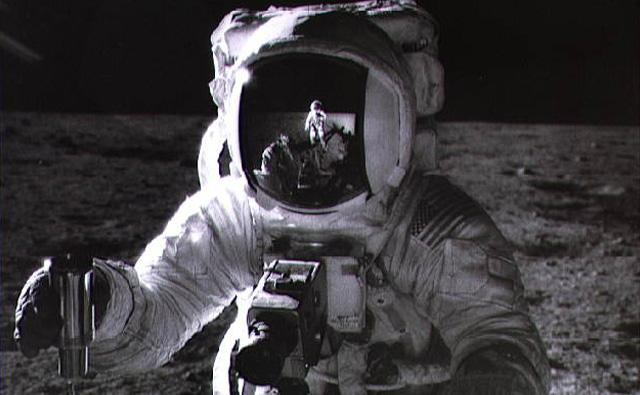
\includegraphics[width=10cm]{apolloman}}
%\pause
%    \subfigure{
%    \includegraphics[width=5cm]{concorde}}
%\pause
%    \subfigure{
%    \includegraphics[width=4.5cm]{enterprise}}
  \end{figure}
\end{frame}

\begin{frame}
\frametitle{A brief history}
\begin{description}
\item[ALGOL68] 1968, 1973 (Revised Report)
\end{description}
\begin{itemize}
\item IFIP WG2.1: Dijkstra, Hoare, Naur, Wirth, McCarthy, Yoneda, Bourne \ldots
\item Core team: Van Wijngaarden, Mailloux, Peck, Koster
\item Two-level grammar
\end{itemize}
\vspace{1cm}
\emph{Compare:}
\begin{description}[align=left]
\item[C] 1967 (BCPL), 1970 (B), 1978 (K\&R), 1989 (ANSI C)
\end{description}
\end{frame}

\begin{frame}
\frametitle{ALGOL68 in a nutshell}
Influence on C/C++
\begin{itemize}
\item \texttt{STRUCT}, safe \texttt{UNION}, references, \texttt{+=}, declare near first use
\end{itemize}
A functional language?
\begin{itemize}
\item Nested, higher-order, and anonymous functions
\item Currying (extension)
\end{itemize}
Programmer-friendly
\begin{itemize}
\item Non-local \texttt{GOTO}, operator overloading, array slices
\item Dangling reference checks, garbage collection 
\end{itemize}
\end{frame}

\begin{frame}
\frametitle{How to write a compiler}
\framesubtitle{Syntax and semantics}
\begin{enumerate}
\item SPL is awful, so fix it
\item Write a recursive decent parser
\begin{itemize}
\item \textbf{Do not use backtracking!}
\end{itemize}
\item Implement a hash table
\item Check types, then unify
\begin{itemize}
\item All type variables must be fully deduced
\item Detect cycles in deduced types
\end{itemize}
\item Write another pretty printer
\begin{itemize}
\item Some assembly required
\end{itemize}
\end{enumerate}
\end{frame}

\begin{frame}[fragile]
\begin{block}{Type checking}
\lstset{language=[68]Algol,basicstyle=\tt\scriptsize,deletekeywords={sign},morekeywords={\%>}, stringize={"}}
\begin{lstlisting}
DECLFUN decl = get fun signature (call);
PARAMS sign = args OF decl;

IF UPB args OF call /= UPB sign THEN
    complain("wrong number of arguments", pos OF call)
ELSE
    FOR i TO UPB args OF call DO
        (args OF call)[i] %> type OF sign[i]
    OD
FI;
\end{lstlisting}
\end{block}
\end{frame}

\begin{frame}
\frametitle{Code generation}
Target architecture: 32bit x86 (Linux)
\begin{itemize}
\item CISC, two-operand instructions
\begin{itemize}
\item \texttt{add \emph{dest}, \emph{src}} 
\end{itemize}
\item 6 general purpose registers
\begin{itemize}
\item Used to hold results of subexpressions
\item Make expressions `left-leaning' to reduce pressure
\end{itemize}
\item I/O using Linux syscalls
\end{itemize}
\end{frame}

\begin{frame}
\begin{block}{Finally}
\begin{itemize}
\item Garbage collection
\end{itemize}
\end{block}
\end{frame}

\begin{frame}
\frametitle{Which technique to use?}
\framesubtitle{Garbage collection}
Reference counting
\begin{itemize}
\item Need to store counter
\item Add code at scope exits, \texttt{=}, \texttt{(,)}, \ldots
\begin{itemize}
\item Requires templating for polymorphic functions
\end{itemize}
\end{itemize}
Garbage collection
\begin{itemize}
\item Determine and reclaim unreachable memory
\item One extra bit for each cell
\end{itemize}
\end{frame}

\begin{frame}[fragile]
\frametitle{Mark \& sweep}
\framesubtitle{Garbage collection}
Reification
\begin{itemize}
\item Expose the internals of SPL
\end{itemize}
\begin{code}
\lstset{language=C, morekeywords={\_stack,\_stackSize}, basicstyle=\tt\scriptsize}
\begin{lstlisting}
Void gc_collect()
{
    Int i = _stackSize();
    while(i > 0) {
        i = i - 1;
        gc_mark(_stack(i));
    }
    gc_sweep();
}
\end{lstlisting}
\end{code}
\end{frame}

\begin{frame}[fragile]
\frametitle{Reification}
\framesubtitle{Garbage collection}
\begin{code}
\lstset{language=C, morekeywords={\_read,\_touch, \_valid, \_reinitHeap, \_reached, \_mkAvail}, basicstyle=\tt\scriptsize}
\begin{lstlisting}
Void gc_mark(Int addr)
{
    while(_valid(addr)) {
        (Int,Int) cell = _read(addr);
        _touch(cell);
        gc_mark(fst(cell));
        addr = snd(cell);
    }
}
\end{lstlisting}
\end{code}
\end{frame}

\begin{frame}[fragile]
\frametitle{Reification}
\framesubtitle{Garbage collection}
\begin{code}
\lstset{language=C, morekeywords={\_read,\_touch, \_valid, \_reinitHeap, \_reached, \_mkAvail}, basicstyle=\tt\scriptsize}
\begin{lstlisting}
Void gc_sweep()
{
    Int i = _reinitHeap();
    while(i > 0) {
        i = i-1;
        if(!_reached(i)) _mkAvail(i);
    }
}
\end{lstlisting}
\end{code}
\end{frame}

\begin{frame}[fragile]
\frametitle{Real world considerations}
\framesubtitle{Garbage collection}
\begin{itemize}
\item What if the heap is \emph{really} full?
\item When to run \texttt{gc\_collect()}?
\end{itemize}
\end{frame}

\begin{frame}
\frametitle{References}
Code available: 
\begin{itemize}
\item \url{https://github.com/squell/algol68-spl}
\end{itemize}

Algol 68 Genie
\begin{itemize}
\item Free software (GPL) by Marcel van der Veer
\item Latest version: 2.6 (November 2012)
\item \url{http://jmvdveer.home.xs4all.nl/}
\end{itemize}
\end{frame}

\appendix
\newcounter{finalframe}
\setcounter{finalframe}{\value{framenumber}}

\begin{frame}[fragile]
\begin{block}{AST}
\lstset{language=[68]Algol,basicstyle=\tt\scriptsize,deletekeywords={op,repr}}
\begin{lstlisting}
MODE SYMBOL  = STRUCT(STRING repr, [2]INT pos);
MODE CONST   = STRUCT(INT int, [2]INT pos);

MODE IDENT   = STRUCT(STRING name, [2]INT pos, 
                      REF DECLINFO info);
MODE MONAD   = STRUCT(SYMBOL op, REF EXPR lhs);
MODE DYAD    = STRUCT(SYMBOL op, REF EXPR lhs, rhs);

MODE TUPLE   = STRUCT(REF EXPR lhs, rhs, [2]INT pos);
MODE FUNCALL = STRUCT(IDENT id, REF[]EXPR args);

MODE EXPR    = UNION(SYMBOL,CONST,MONAD,DYAD,
                     TUPLE,IDENT,FUNCALL);
\end{lstlisting}
\end{block}
\end{frame}

\begin{frame}[fragile]
\begin{block}{Parsing}
\lstset{language=[68]Algol,basicstyle=\tt\scriptsize,deletekeywords={lt}}
\begin{lstlisting}
OP MATCH = (REF TYPE spec)BOOL:
BEGIN
    IDENT id;
    IF MATCH id THEN
        spec := id; TRUE
    ELIF MATCH "(" THEN
        HEAP TYPE lt, rt;
        REQUIRE lt;
        REQUIRE ",";
        REQUIRE rt;
        spec := PAIRT(lt, rt);
        REQUIRE ")"; TRUE
    ELSE
        FALSE
    FI
END
\end{lstlisting}
\end{block}
\end{frame}

\begin{frame}[fragile]
\begin{block}{Code generation}
\lstset{language=[68]Algol,basicstyle=\tt\scriptsize,deletekeywords={then,if,else,false,skip},morekeywords={THEN,IF,ELSE,FALSE,ISNT,TRUE,OF,FI,\%},sensitive=true}
\begin{lstlisting}
LABEL kick start = obtain label;
LABEL false = obtain label;
elaborate (cond OF if, TRUE, kick start, false);
emit label (kick start);
%then OF if;
IF else OF if ISNT NIL THEN
    LABEL skip = obtain label;
    emit jump (skip, unconditional);
    emit label (false);
    %else OF if;
    emit label (skip)
ELSE
    emit label (false)
FI
\end{lstlisting}
\end{block}
\end{frame}


\setcounter{framenumber}{\value{finalframe}}

\end{document}
